\subsection{Protótipo e experimento em campo}
\label{subsec:prototipoExperimento}

Um protótipo foi desenvolvido para avaliar o uso dos agentes fora do ambiente virtual. O objetivo desta fase é recolher dados sobre a latência e taxa de perda do agente. A latência é importante para alguns tipos aplicações como por exemplo para detectar colisão \cite{santanaMestrado:2014}. Assim, essas informações são importantes para identificar quais os tipos de aplicações os agentes são melhores empregados. Uma rede para ser bem sucedida com a utilização dos agentes de software necessita mante-los ativo até o fim de sua missão.A Figura \ref{fig:noInstaladoVeiculo} pode-se visualizar um nó instalado em um veículo.

\begin{figure}[htbp]
	\centering
	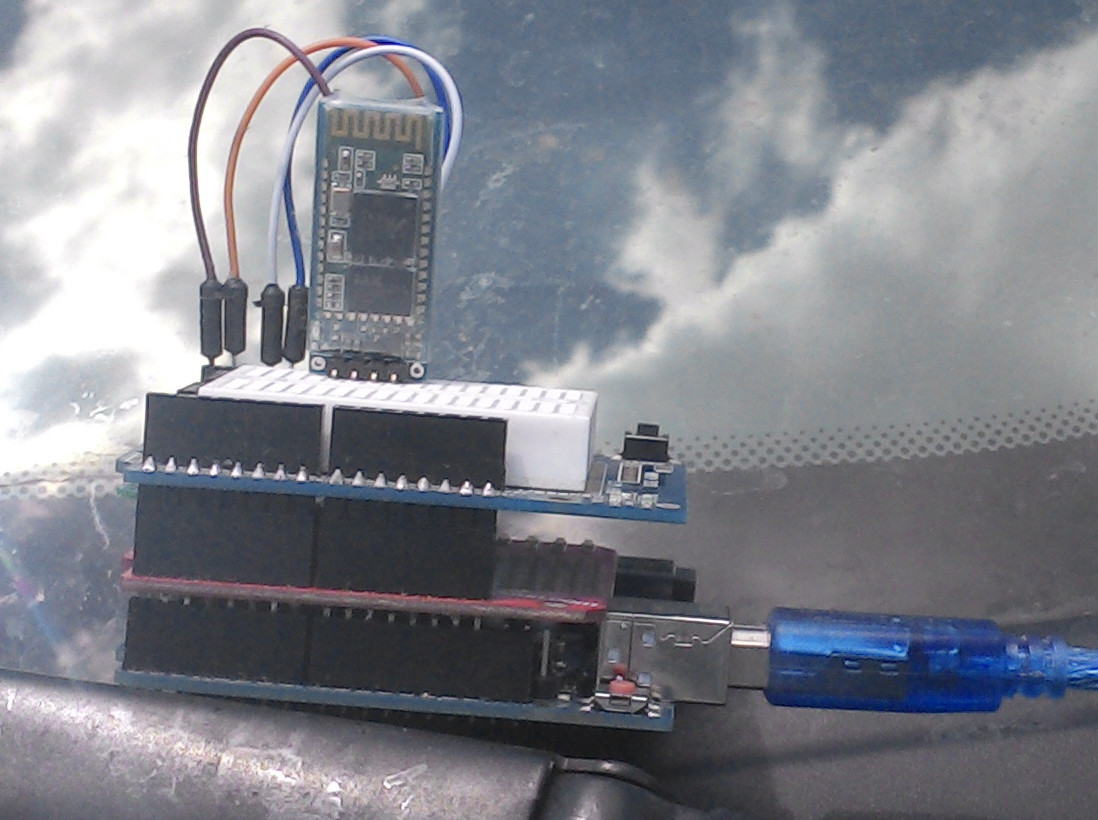
\includegraphics[scale=0.06]{metodologia/figuras/noInstaladoVeiculo.jpg}
	\caption{Nó instalado em um veículo.}
	\label{fig:noInstaladoVeiculo}
\end{figure}

O experimento utiliza três nós, onde dois nós são para os veículos e um desempenha o papel de infraestrutura. A estrutura dos nós foi reaproveitada do trabalho \cite{santanaMestrado:2014}. Os equipamentos necessários para a construção dos nós podem ser visualizados na Tabela \ref{tab:componentesPrototipo}. 

\begin{table}[ht]
	\caption{Equipamentos utilizados no experimento.}
	\centering
	\begin{tabular}{|l|l|}
		\hline
		Equipamento & Quantidade \\ \hline
		Notebook & 1 \\ \hline 
		Módulo bluetooth modelos JY-MCU & 2 \\ \hline
		Arduíno UNO & 2 \\ \hline
		Xbee shield & 2 \\ \hline
		Mini protoboard 170 pontos & 2 \\ \hline
		Xbee S1 & 3 \\ \hline
		XBee Explorer USB Adapter & 1 \\ \hline 
		Motorola RAZR I & 1 \\ \hline
		Motorola Moto G & 1 \\ \hline
	\end{tabular}
	\label{tab:componentesPrototipo}
\end{table}

Ao iniciar o experimento é introduzido um agente em um dos nós. Então o agente deve migrar sempre que encontrar um outro nó.

\subsubsection{Arquitetura do nó}

A Figura \ref{fig:arquiteturaPrototipoInfraestrtura} demonstra a arquitetura da infraestrutura que utiliza um Xbee e um XBee Explorer USB Adapter conectado em um notebook.

\begin{figure}[htbp]
	\centering
	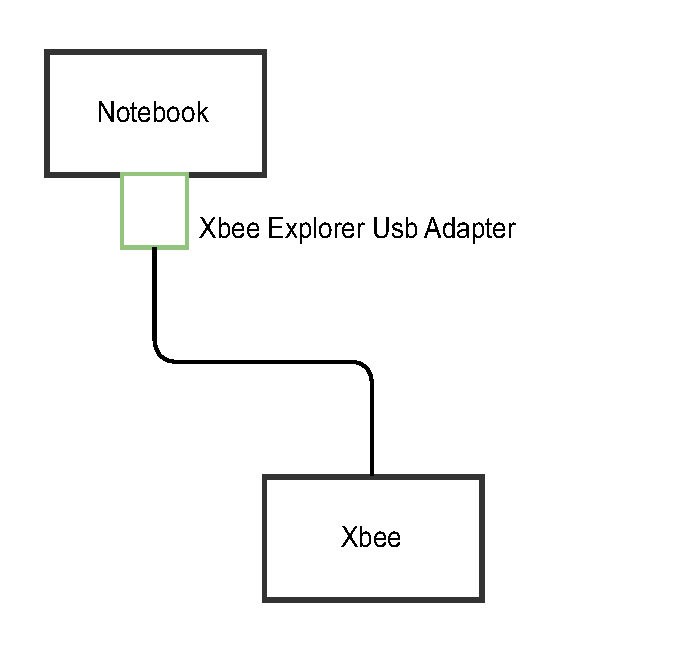
\includegraphics[scale=0.5]{metodologia/figuras/arquiteturaPrototipoInfraestrtura.pdf}
	\caption{Arquitetura da infraestrutura.}
	\label{fig:arquiteturaPrototipoInfraestrtura}
\end{figure}

O agente fica hospedado no smartphone, o arduino serve somente como interface entre o smartphone e o módulo Xbee. A comunicação entre o arduino e o smartphone acontece através do bluetooth. 

O smartphone acolhe o agente por que possui um ambiente mais rico em recursos do que o arduino, isto significa que o smartphone possui GPS, mais memória e outros recursos para que o agente possa desempenhar a sua missão, a Figura \ref{fig:arquiteturaPrototipoVeiculo} ilustra a estrutura do nó que atua nos veículos. 

\begin{figure}[htbp]
	\centering
	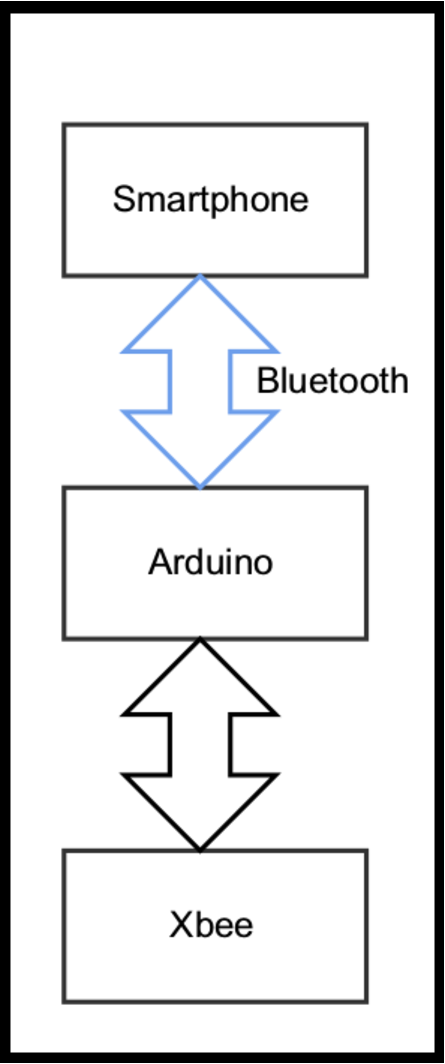
\includegraphics[scale=0.5]{metodologia/figuras/arquiteturaPrototipoVeiculo.pdf}
	\caption{Estrutura do nó no veículo.}
	\label{fig:arquiteturaPrototipoVeiculo}
\end{figure}

Para sincronizar o relógio dos smartphones utilizados no experimento foi utilizado o aplicativo NTPSync (\cite{Ntpsync:2015}), que é um aplicativo simples para sincronizar o tempo. Manter o relógio sincronizado é importante para medir a latência com precisão. 


Para hospedar o agente foi desenvolvido um aplicativo Android, esse aplicativo fornece ao agente os mecanismos necessários para realizar a sua missão. Através dele o agente consegue acessar o GPS, o bluetooth e a tela do smartphone. No display do aplicativo tem um alerta que informa se existe algum agente hospedado no smartphone e um botão para criar novos agentes. A Figura \ref{fig:appScreen} demonstra a tela do aplicativo responsável pelo agente.

\begin{figure}[htbp]
	\centering
	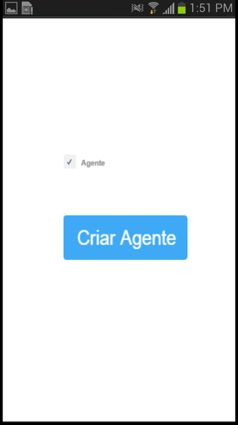
\includegraphics[scale=0.5]{metodologia/figuras/appScreen.jpg}
	\caption{Tela do aplicativo.}
	\label{fig:appScreen}
\end{figure}

Esse aplicativo também realiza a coleta dos dados em arquivo. Os dados coletados são a hora que o agente migrou, a hora que recebeu um agente em milisegundo. Então para calcular a latência é a subtração da hora de quando o novo hospede recebeu o agente e a hora que o agente iniciou a migração no antigo hospede.

\subsubsection{Agente}

A missão do agente neste experimento é migrar sempre que encontrar um novo nó. O agente deve transportar as instruções, o identificador da migração e a posição do antigo nó hospede para o novo nó. As instruções utilizadas pelo agente são apresentadas na Tabela \ref{tab:instrucoesAgente}, elas são formadas por uma letra maiúscula, uma sequência de três letras minúscula e um número, esse padrão é utilizado pelo mecanismo de validação e recuperação. Para delimitar o fim da instrução é utilizado o caractere de ponto e vírgula (\emph{;}). O identificador da migração é um número que serve para auxiliar no cálculo de latência. Assim com o identificador é possível encontrar a hora que o agente migrou e a hora que o agente foi recebido por completo no hospedeiro em dois arquivos diferentes. Sempre antes do agente migrar o identificador de migração é incrementado.  

\begin{table}[ht]
	\centering
	\begin{tabular}{ | l | l |}
		\hline
		Instrução &  Ação \\ \hline
		Spap1 & solicitar e armazenar no agente a posição atual para o nó hospedeiro.\\ \hline
		Remi2 & realizar migração.\\ \hline
		Bnov3 & buscar nós vizinhos. \\ \hline 
	\end{tabular}
	\caption{Lista de instruções}
	\label{tab:instrucoesAgente}
\end{table}

O agente é formado por dois elementos, como demonstra a Figura \ref{fig:estruturaAgente}. O primeiro elemento denominado \emph{cabeçalho} é a região onde estão as instruções. O \emph{corpo} é o elemento onde os dados do agente são armazenados. O corpo é envolvido pelos caracteres de colchetes (\emph{[ ]}), essa estrutura é utilizado para separar o cabeçalho do corpo.

\begin{figure}[htbp]
	\centering
	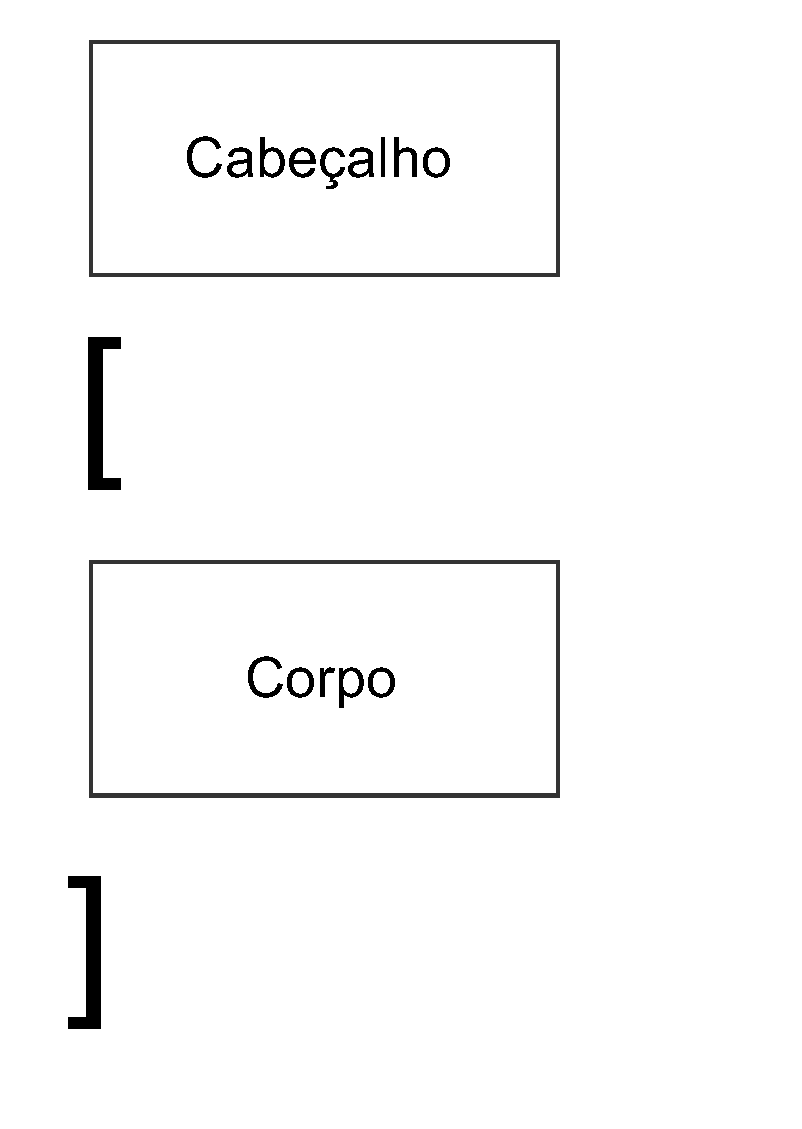
\includegraphics[scale=0.25]{metodologia/figuras/estruturaAgente.pdf}
	\caption{Nó instalado em um veículo.}
	\label{fig:estruturaAgente}
\end{figure}

\subsubsection{Mecanismo validação e recuperação}

Após um nó receber o último colchete (\emph{]}) ou 500 ms com um agente incompleto o mecanismo de validação e recuperação é ativado. A principal função deste mecanismo é tentar recuperar o agente danificado e se não conseguir descarta-lo. 

A validação verifica se todas as instruções têm cinco caracteres, se a primeira letra é maiúscula e o último caractere é um número, além de verificar as instruções ele válida a estrutura do corpo. Quando alguma instrução não atende uma das três características mencionadas anteriormente ou o corpo não atende o padrão, o mecanismo de recuperação entra em ação. 

Se o erro for no \emph{cabeçalho}, o algoritmo verifica o tamanho da instrução se for maior que cinco ele descartar o agente. Se for menor ele confere a primeira letra se ela atender algumas das instruções suportadas ele recupera colocando a instrução correta. Se não conseguir através do primeiro caractere a próxima tentativa é o último caractere que deve ser um número. Se nenhuma das tentativas forem alcançadas o agente é descartado. A Figura \ref{fig:estruturaInstrucao} demonstra a estrutura da instrução utilizado neste trabalho.

\begin{figure}[htbp]
	\centering
	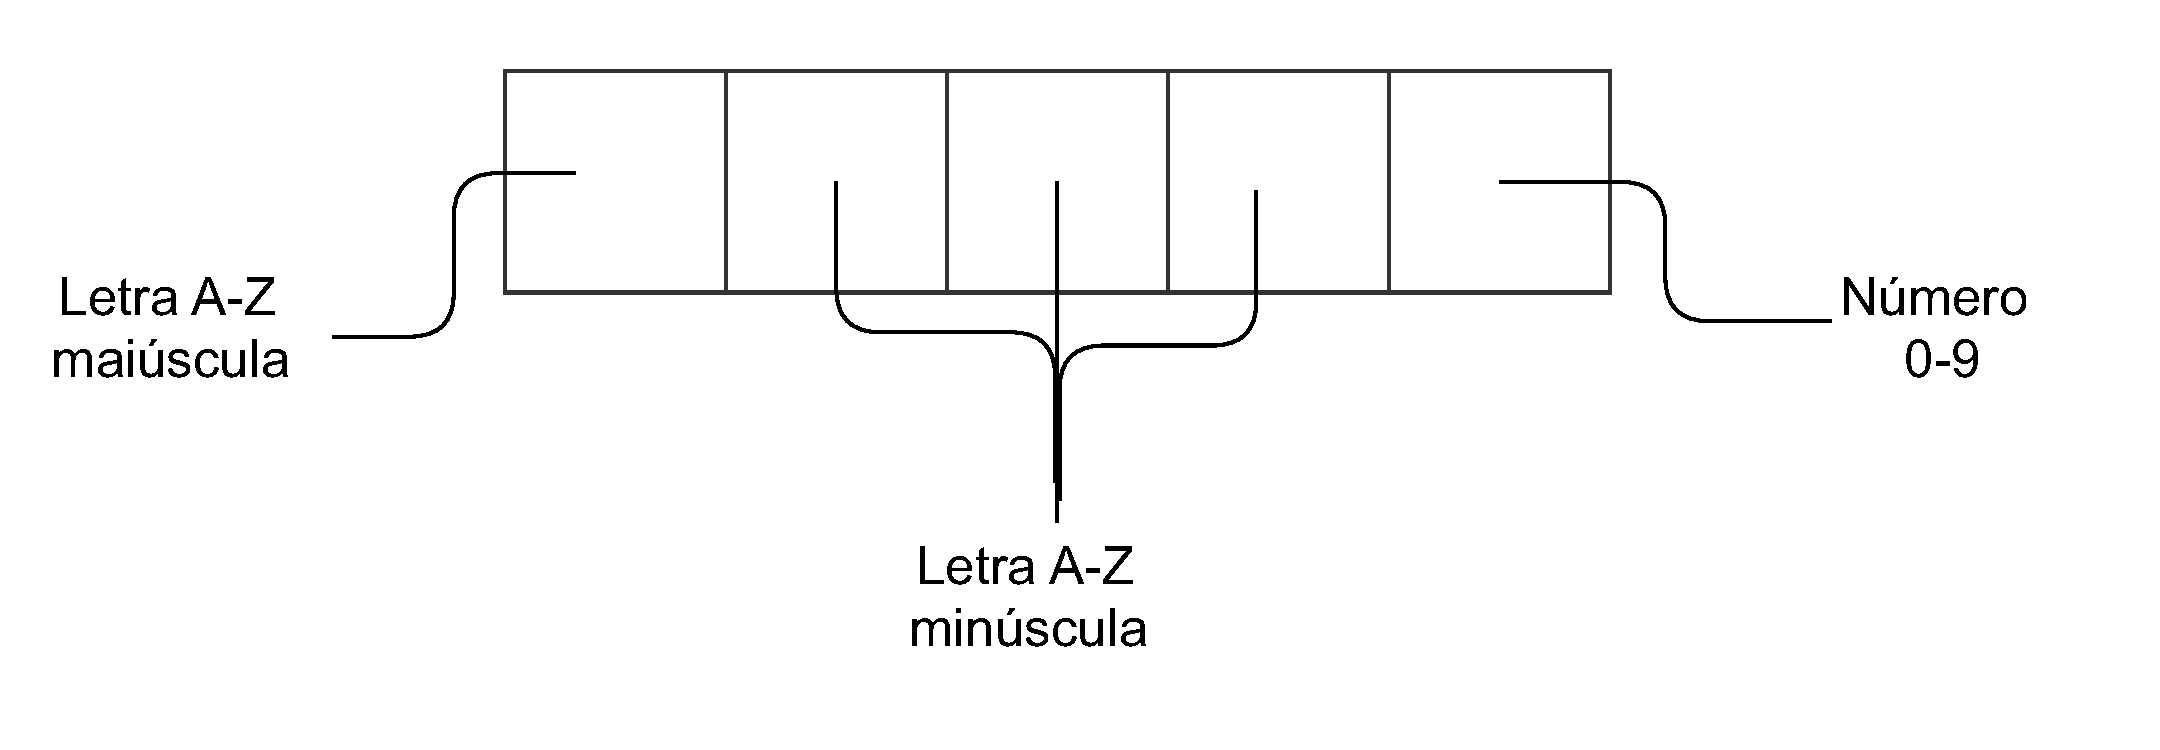
\includegraphics[scale=0.27]{metodologia/figuras/estruturaInstrucao.pdf}
	\caption{Estrutura da Instrução.}
	\label{fig:estruturaInstrucao}
\end{figure}

Para tentar recuperar o corpo, primeiro verifica se existe um caractere de colchete (\emph{[}) iniciando o corpo, se não existir o agente é descartado. Se existir é verificado se o último caractere é um colchete finalizando a estrutura, se não existir o mecanismo coloca o caractere que representa fim. Esse roteiro é reproduzido pelo Algoritmo \ref{lst:mecanismoValidacaoRecuperacao} e a Figura \ref{fig:exemploCodigoAgente} apresenta o agente utilizado neste trabalho.

\begin{algorithm}
	\scriptsize
	\Inicio{
		\Entrada{Agente}
		$instrucoes = agente.pegarInstrucoes()$\;
		$i \gets 0$\;

		\uIf{agente.contem([)}{
			\Repita{$i < instrucoes.quantidade$}{
				$instrucao \gets instrucao[i]$ \;
				\uIf{$instrucao.tamanho < 5$}{
					\uIf{verificar(instrucao.primeiroCaracter)}{
						$instrucao \gets recuperar(instrucao.primeiroCaracter)$\;
					}
					\Else{
						\uIf(verficar(instrucao.ultimoCaracter)){
							$instrucao \gets recuperar(instrucao.ultimoCaracter)$\;
						}
						\Else{
							agente.remover()\;
						}
					}
					
				}
				\Else{
					agente.remover()\;
				}
				i++\;
			}
			\uIf{$agente.ultimoCaracter \neq ]$}{
				$agente.ultimoCaracter \gets ]$
			}
		}
		\Else{
			agente.remover()\;
		}
	}

		
	\caption{Mecanismo validação e recuperação.}
	\label{lst:mecanismoValidacaoRecuperacao}
\end{algorithm}

\begin{figure}[htbp]
	\centering
	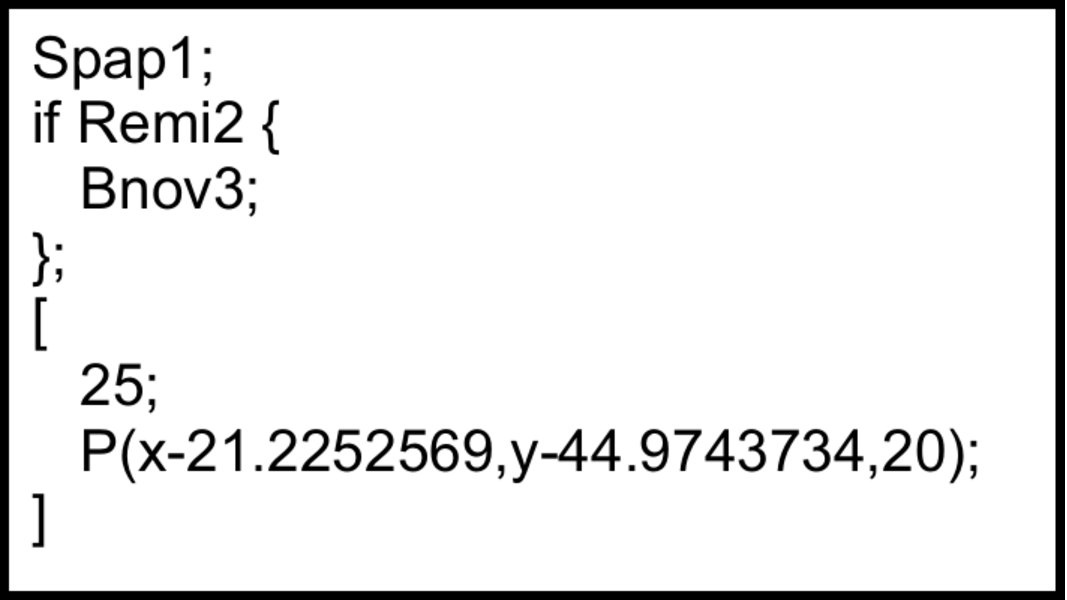
\includegraphics[scale=0.3]{metodologia/figuras/exemploCodigoAgente.pdf}
	\caption{Agente Software.}
	\label{fig:exemploCodigoAgente}
\end{figure}

\subsubsection{Trajeto e cenário}

Como trajeto é utilizada a avenida norte que está localizada no campus da Universidade Federal de Lavras. O trajeto pode ser visualizado na Figura \ref{fig:trajetoExperimento}. Nesse trajeot o veículo percorre 344,45 metros. 

\begin{figure}[htbp]
	\centering
	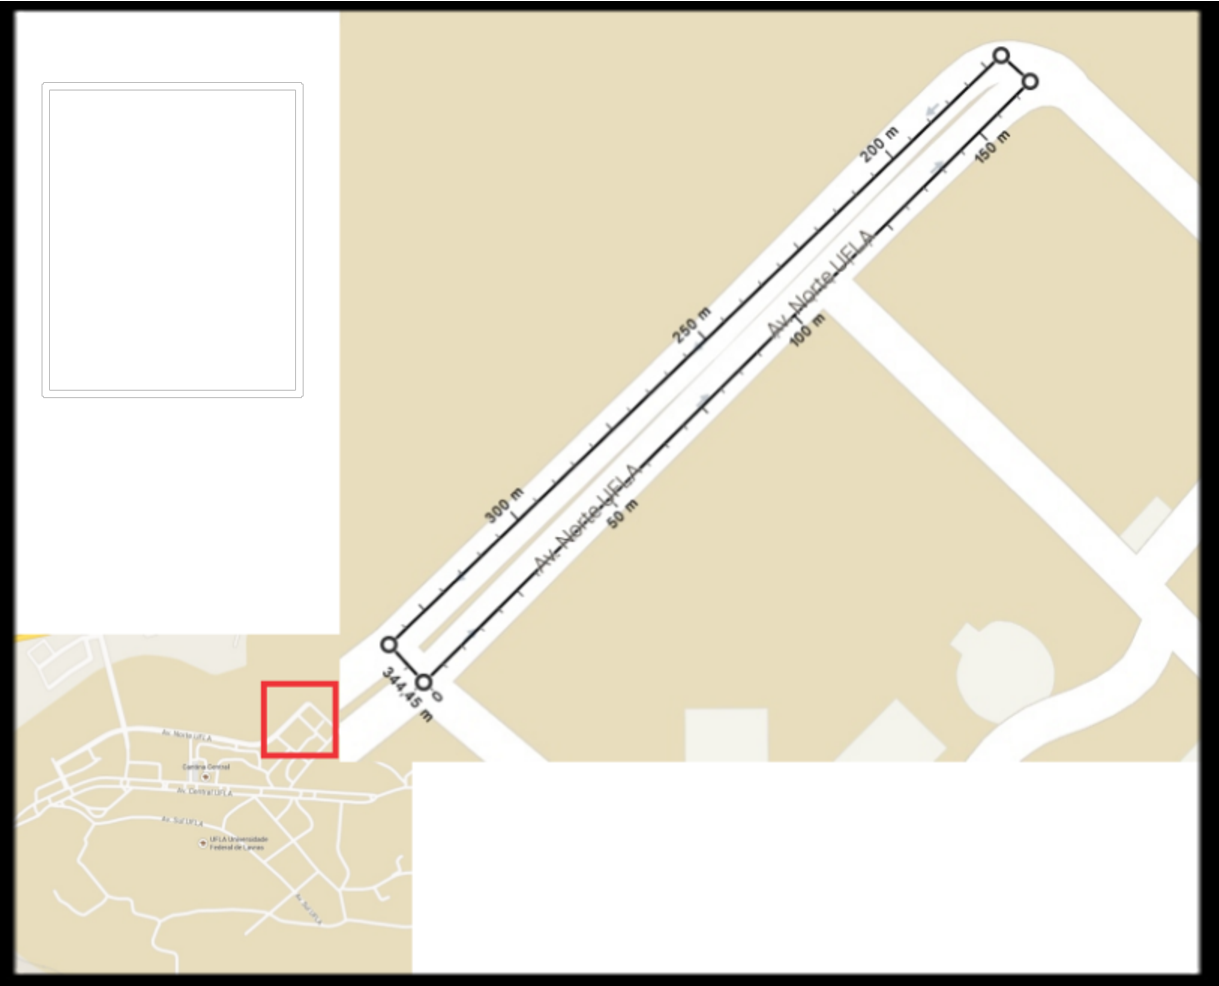
\includegraphics[scale=0.4]{metodologia/figuras/trajetoExperimento.pdf}
	\caption{Modelo de cidade utilizado.}
	\label{fig:trajetoExperimento}
\end{figure}

Os veículos trafegam sobre o roteiro em velocidade média de 20 km/h, a Figura \ref{fig:veiculosUtilizadoExperimento} pode-se visualizar os veículos utilizados no experimento. Existem dois cenários para realizar o experimento, sendo o primeiro caso com infraestrutura e outro somente com veículos. A infraestrutura está localizada ao centro do trajeto como demonstra a Figura \ref{fig:infraestruturaUtilizadoExperimento}.

\begin{figure}[htbp]
	\centering
	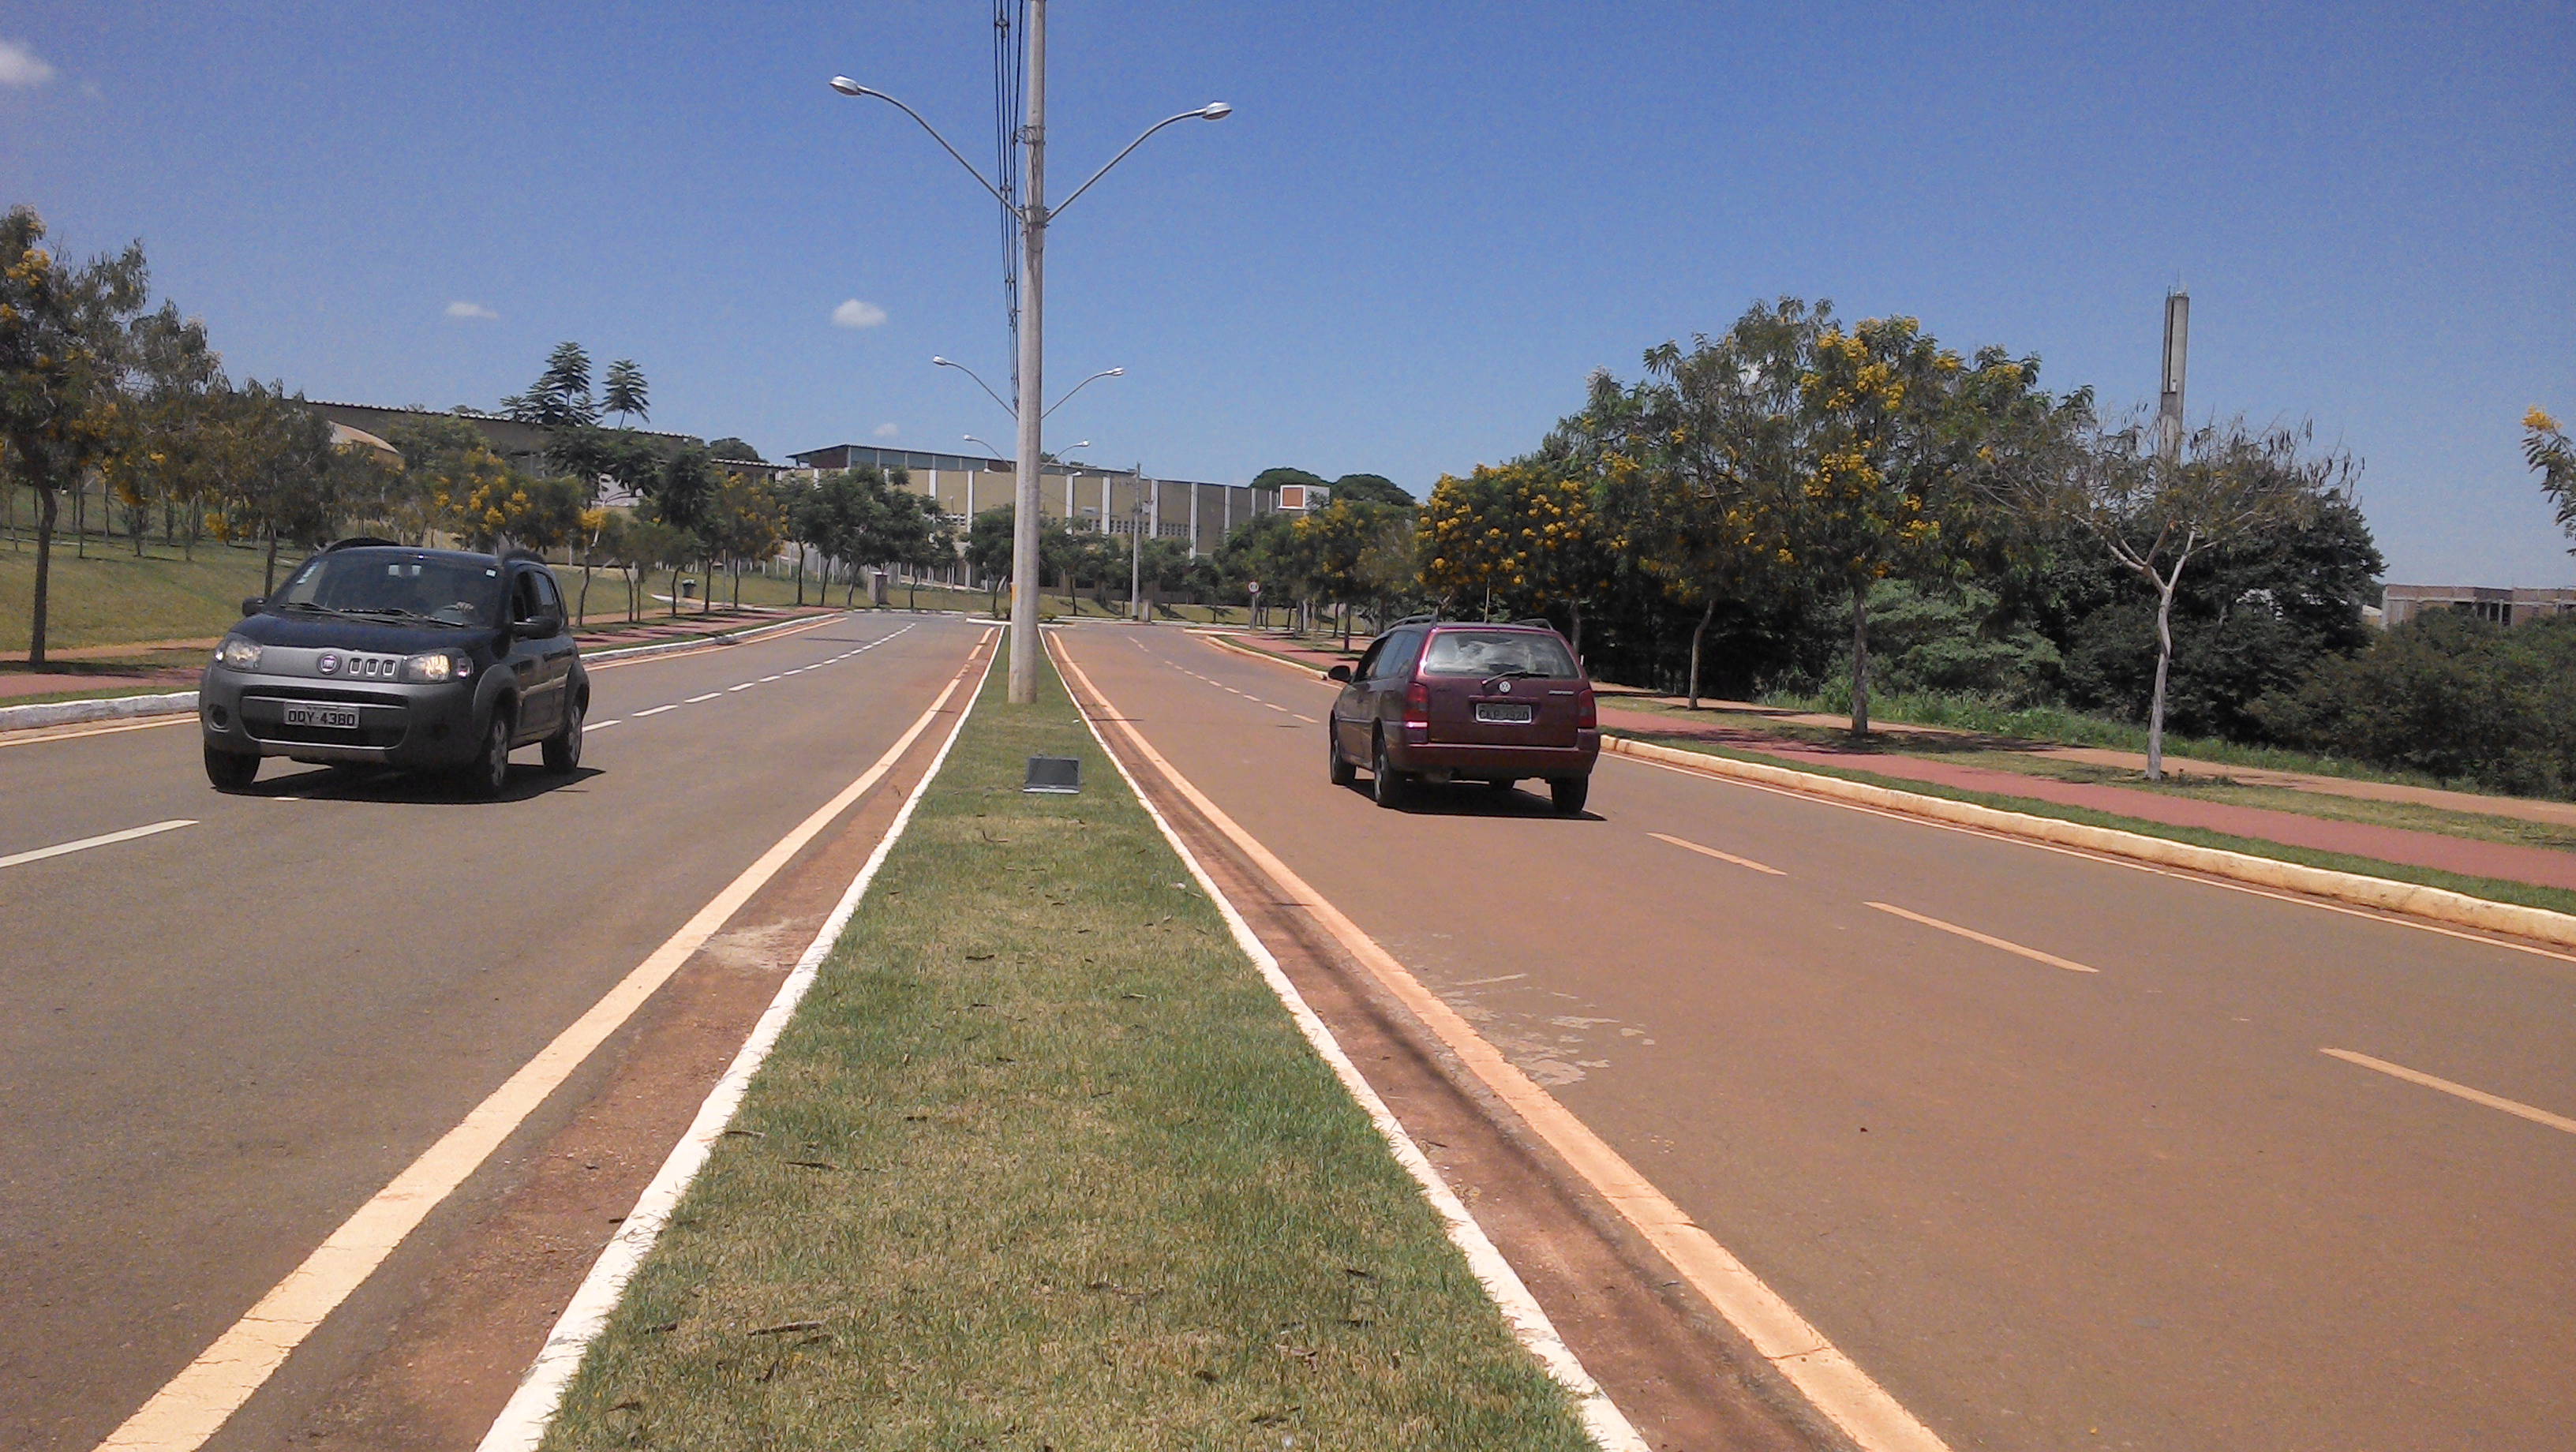
\includegraphics[scale=0.06]{metodologia/figuras/veiculosUtilizadoExperimento.jpg}
	\caption{Veículos utilizados no experimento.}
	\label{fig:veiculosUtilizadoExperimento}
\end{figure}

A infraestrutura é colocada aproximadamente ao centro do cenário. Quando a infraestrutura não é utilizada ela é desligada. A infraestrutura tem a função de receber e armazenar o agente até um novo nó se aproximar. Para saber que o agente passou pela infraestrutura é adicionado um caractere \emph{I} ao corpo do agente. Esse caractere vai auxiliar no cálculo da quantidade de vezes que o agente passou pela infraestrutura.

\begin{figure}[htbp]
	\centering
	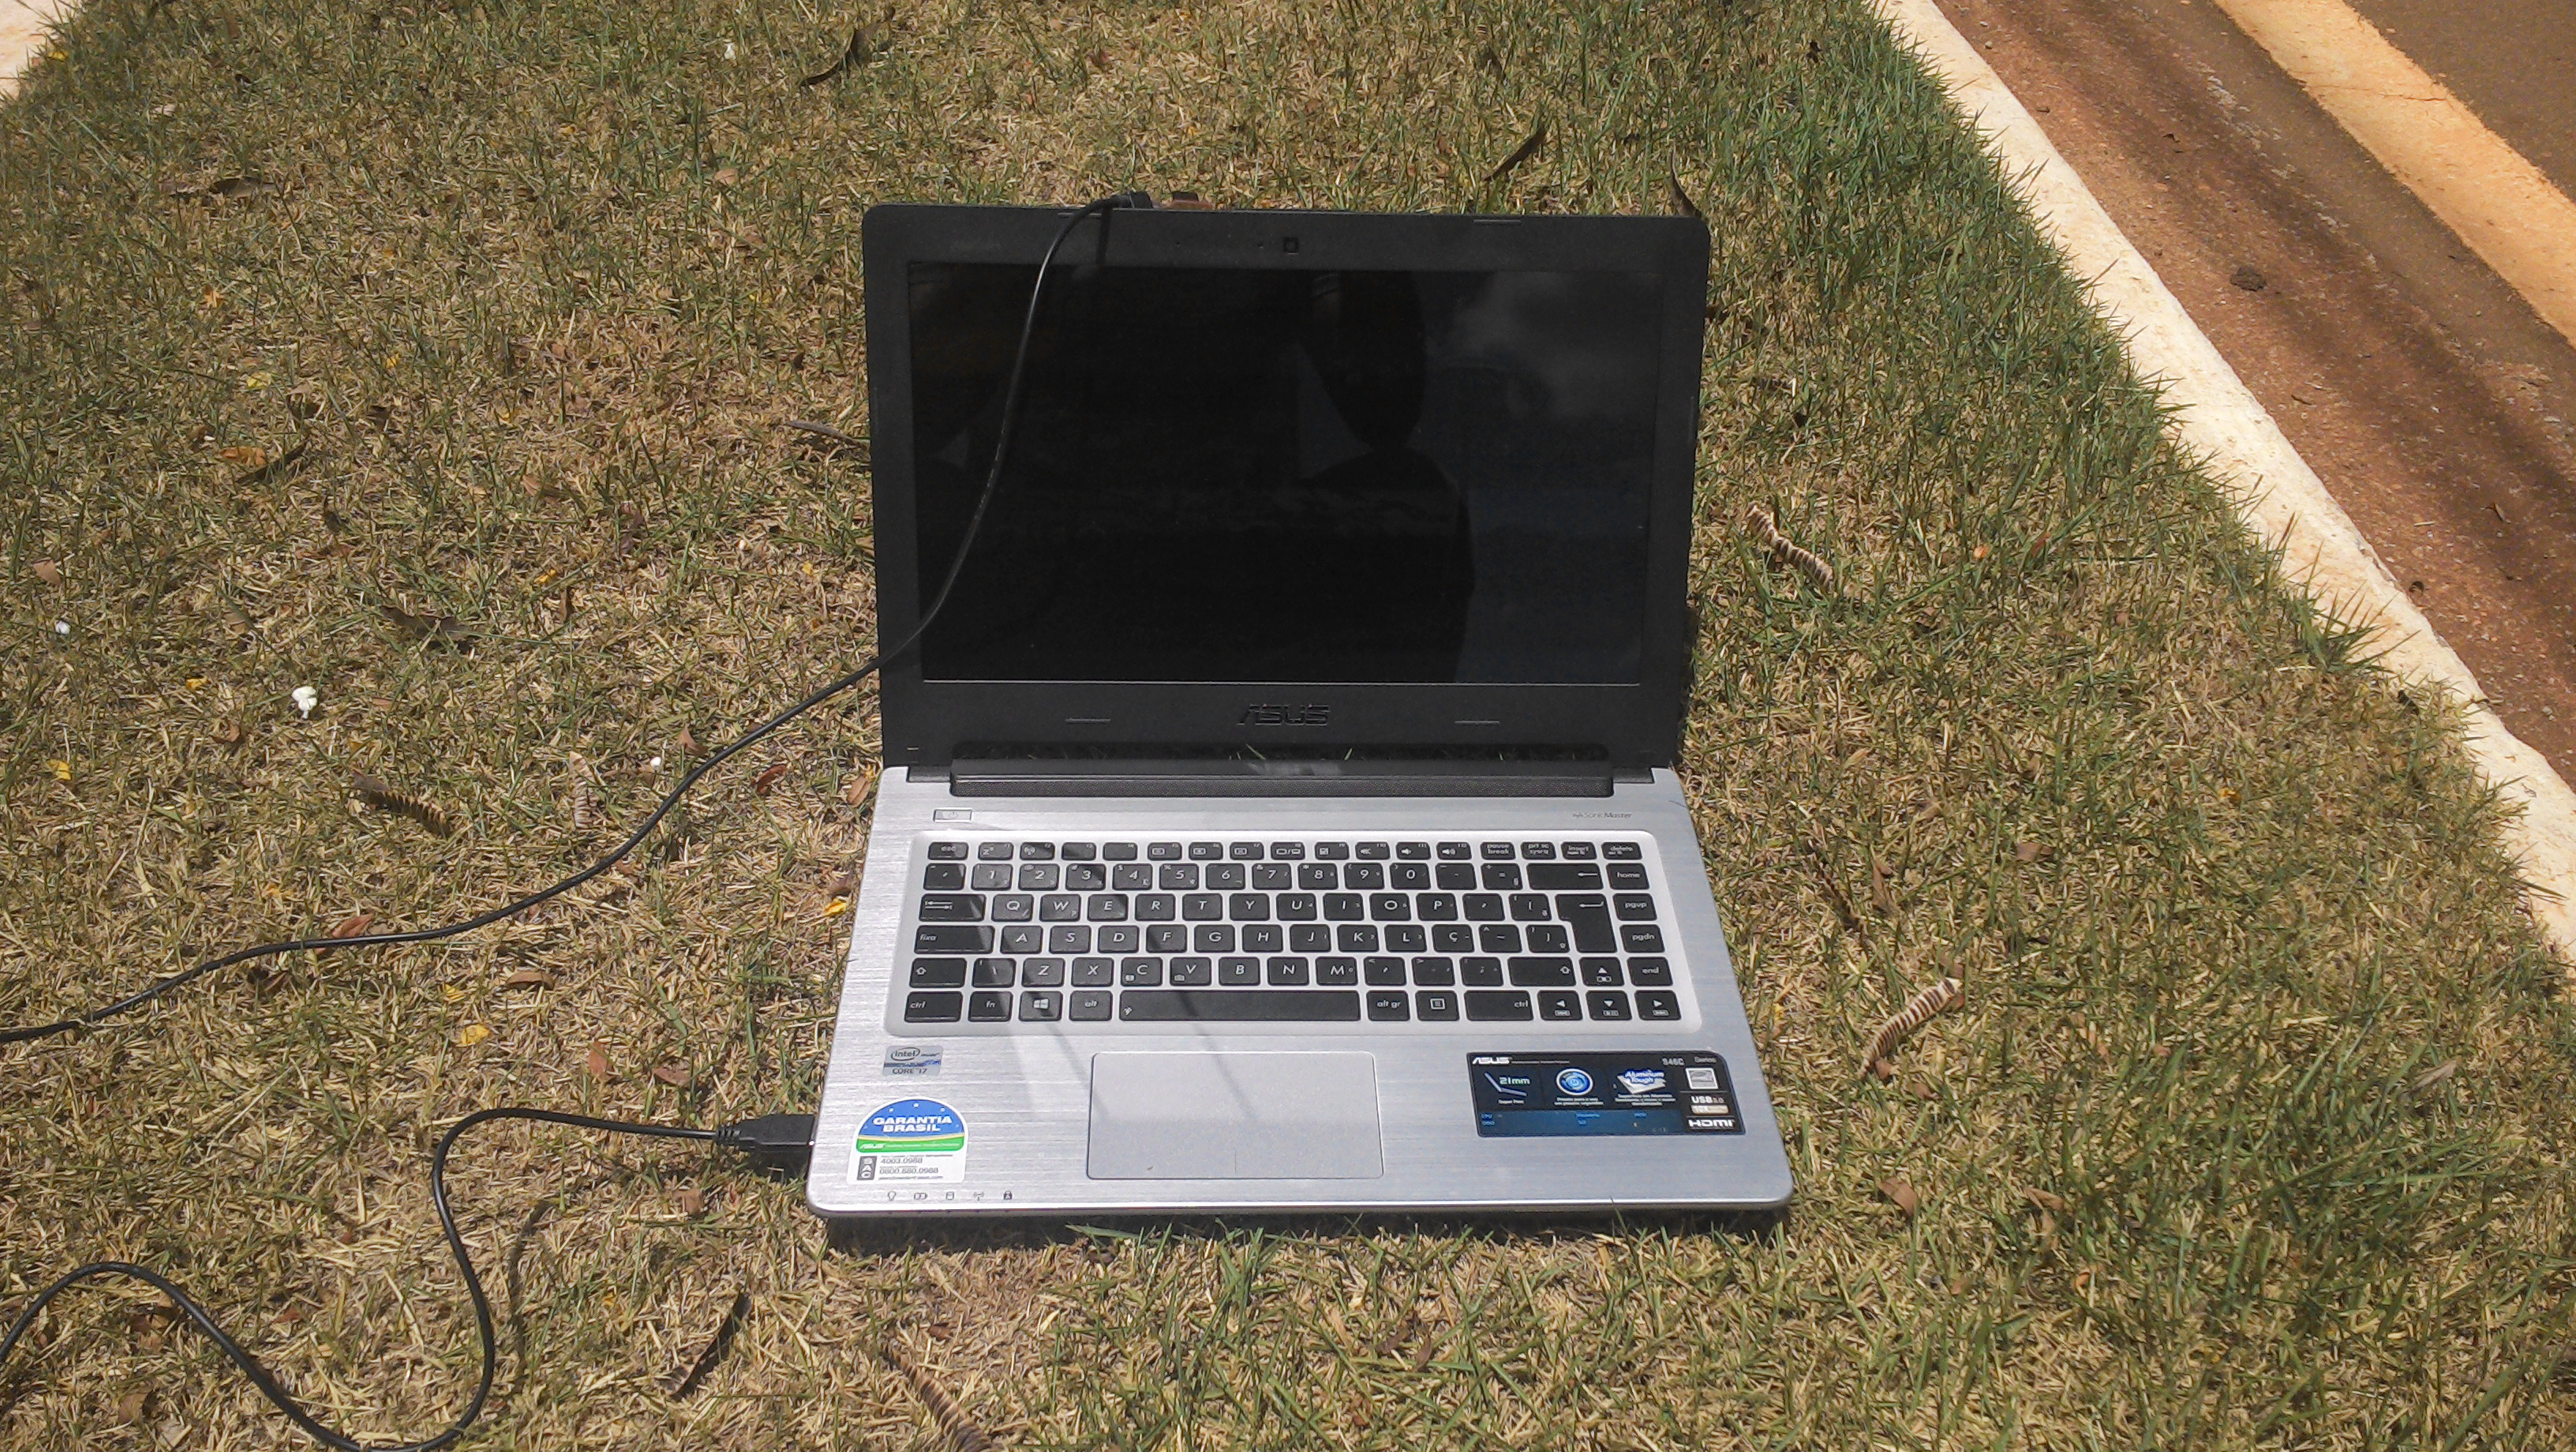
\includegraphics[scale=0.06]{metodologia/figuras/infraestruturaUtilizadoExperimento.jpg}
	\caption{Infraestrutura utilizada no experimento.}
	\label{fig:infraestruturaUtilizadoExperimento}
\end{figure}

No experimento realizado, cada veículo percorreu cinquenta vezes o trajeto, vinte e cinco com a infraestrutura ativada e vinte e cinco com a infraestrutura desativada. Foram recolhidas informações sobre a latência e taxa de perda do agente. Ao fim dessa fase foram calculados o desvio padrão, variância e os resultados foram analisados.
